\documentclass[12pt]{report}
\usepackage[margin=1in]{geometry}
\usepackage{color}
\usepackage{graphicx}
\usepackage{float}

\title{Response to Reviewer 1}

\begin{document}



\author{Andrew PJ Stanley and Andrew Ning}

\maketitle

Thank you for your thorough review of the manuscript and for your comments! We will address each of your comments and questions individually.

\bigskip
Question/Comments are in black.

\color{blue} The corresponding responses are immediately below in blue.

\bigskip \color{black}
**** General comments

\bigskip \color{black}
In the abstract the authors should mention under which conditions the 2 to 5\% reduction was obtained (which spacing, wind shear, etc) and mention the benefit is larger when the inter turbine spacing is smaller.

\color{blue} The abstract was changed to reflect this comment.

\bigskip \color{black}
Mention in the abstract that only two turbine designs are allowed in the optimization procedure in a fixed one to one ratio. Now the abstract gives the impression the turbine design is changed for each turbine.

\color{blue} The abstract was changed to reflect this comment.

\bigskip \color{black}
In several places the authors mention that certain modeling choices were given by the need to restrict the computational time used by the optimization procedure.

\color{blue} Yes, some modeling choices were made to restrict time. In an optimization framework where a model will be called several times every iteration, computationally expensive models become infeasible.

\bigskip \color{black}
Page 3: What is the wake profile in the FLORIS model? The authors define the wake interaction model in detail, but do not provide any details on the actual wake model. Please also use L only for one thing.

\color{blue} An explanation was added about how the version of FLORIS that we used was modified to consider the 3-D flow field. All of the details of the FLORIS modeled were not re-presented here as they are detailed in the cited papers and are used exactly as defined in those papers
%\begin{figure}[H]
  %\centering
  %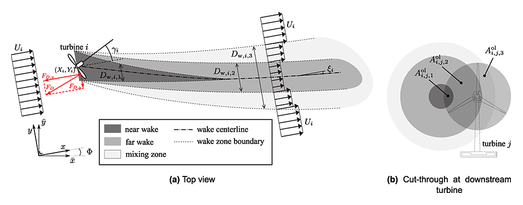
\includegraphics[width=\textwidth]{florisProfile}
%\end{figure}
Also, the equation was adjusted to clarify total loss and individual loss from each turbine.

\bigskip \color{black}
Page 7 cost model: The authors refer to a reference that is not yet available to the referee. Without access to this paper it is impossible to see what the authors exactly did. If the paper will appear soon there is no need to repeat things here if all is identical, but for the moment this cannot be checked.

\color{blue} Yes this is unfortunate. We expect this paper to be published soon, in the meantime we will attach a pre-print version of the paper!

\bigskip \color{black}
Page 7 section 2.6: The authors say it does not matter too much how many different groups are used, but no actual numbers are mentioned. Please provide these numbers to back up this statement.

\color{blue} Relating to the last comment, the intention is that the reader would refer to the citation for the specifics on this topic. We will attach a pre-print version of the paper.

\bigskip \color{black}
page 9 last section (also page 11 top): I found the description of the ``spacing multiplier'' very confusing. Figure 8 helps a lot, but the text in the mentioned paragraph
should be clarified.

\color{blue} This portion was reworked for additional clarity.

\bigskip \color{black}
page 14 first section: Did the authors try to see what happens when they use the turbine designs obtained a a training wind farm as input for the actual optimization algorithm. How close would the result be to the coupled optimization approach? Obviously the coupled optimization approach always gives a better results (assuming obviously that the model would be perfect), but how much is the difference? In the results we namely also see that for very small spacings the "sequential turbine design then layout" is worse than just using the "layout" optimization. Is this because the reference turbines are already somewhat optimized to be located in a wind farm? And would a better design of more appropriate reference turbines reduce the benefit of the coupled optimization approach?

\color{blue} Excellent point! We added a paragraph to the end of the conclusion that includes a recommendation for future research to include the consideration of a ``training farm'' for sequential optimization. As for the sequential optimization being worse for very small spacings, yes that is correct. When the turbine is optimized in isolation, it is optimal to be large because it is always exposed to the high free stream wind speeds. In a farm, especially the small farm, the wind speeds that the turbine actually is exposed to are much lower from wake interference, so in these cases it is more optimal to be smaller. It happens that the baseline design is close to the optimal turbine for the closely spaced wind farm, which makes it more optimal than the larger sequential optimization. 

\bigskip \color{black}
How exactly does this work compare to earlier work by the same authors, i.e. Stanley, A. P. J., Thomas, J., Ning, A., Annoni, J., Dykes, K., and Fleming, P., “GradientBased Optimization of Wind Farms with Different Turbine Heights,” Wind Energy Symposium, Grapevine, TX, AIAA, Jan. 2017. doi:10.2514/6.2017-1619 Stanley, A. P. J., Ning, A., and Dykes, K., “Benefits of Two Turbine Rotor Diameters and Hub Heights in the Same Wind Farm,” Wind Energy Symposium, Kissimmee, FL, Jan. 2018. doi:10.2514/6.2018-2016 These papers are not referenced at the moment, but seem to follow for a big part the optimization philosophy outlined here, with the present work focusing on the coupled layout wind turbine design approach. It may be possible to compare the results obtained here with the previous results.

\color{blue} These papers were added and explained in the literature review! This paper is the culmination of these two conference papers and the referenced journal submission.

\bigskip \color{black}
Can the authors compare their optimization results with methods already presented in the literature?

\color{blue} We feel like we have made significant enough improvements that direct comparison of the results of our paper with those in the mentioned literature (beyond the mention that our study as well as the literature show benefits to mixed turbine wind farms) is not necessary. The purpose of this paper is not to replicate any of their research, but to build on it.

\bigskip \color{black}
The authors only show results of the turbine designs obtained using the optimization. I would also be interested in seeing the corresponding wind farm layouts of the most optimal configuration that was found.

\color{blue} We considered this at some length before the original submission, and decided to leave out the optimal wind farm layouts simply due to the shear number of figures it would require. For each wind farm, there are 3 spacing multipliers considered, and for each spacing multiplier there are 3 shear exponents. Then there are 4 optimizations that were run (layout, sequential, coupled with one group, coupled with two groups). That is a total of 72 layout plots to include all of the relevant results. To include one or two layouts would not be interesting, because the important part is the comparison between each case, we thus decided to leave them out. 

Although they won't fit in this paper, we have posted the figures and added this link to the paper: 


\bigskip \color{black}
**** Specific comments

\bigskip \color{black}
Page 1: References on the mentioned gradient-free and gradient-based optimization methods are missing.

\color{blue} We double checked the references and they appear to be listed (lines 9-11 on pg 2).

\bigskip \color{black}
Page 2: in this study for additional improvements. -$>$ It should read "in the presented approach" as the authors do not actually consider yaw optimization in this study.

\color{blue} This change was made.

\bigskip \color{black}
Page 2-3: Please clarify the numbers presented here, i.e. the increases in production / reduction in the cost of energy are determined with respect to some reference case, but not for all cases the respective reference cases are clearly defined.

\color{blue} The missing reference case was added.

\bigskip \color{black}
Page 4: Rotation of each wind turbine -$>$ rotation of the blades

\color{blue} This change was made.

\bigskip \color{black}
Page 4: Please define x in equation 5.

\color{blue} ``x'' was changed to ``V'' to represent wind speed.

\bigskip \color{black}
Page 4: The direction data we had -$>$ Please provide the appropriate references / explain. I assume most of the data in figure 5/6 is actually obtained from some literature reference.

\color{blue} Appropriate references were added!

\bigskip \color{black}
Page 5 line 20: Maybe I missed it, but please give the airfoil used in this work.

\color{blue} The source with the airfoils used was added.

\bigskip \color{black}
Page 5 figure 1: Please provide units of Frequency shown here.

\color{blue} Frequency refers to the probability and is unit-less.

\bigskip \color{black}
Page 6 line 1: What 10 groups are used?

\color{blue} The groups were randomly selected as is typical in k-fold cross-validation.

\bigskip \color{black}
Page 6 figure 2: Please give the appropriate units in the figure.

\color{blue} The axes have been normalized and are thus unit-less.

\bigskip \color{black}
Page 8 equation 6: What is D\_rotor? In the optimization both D1 and D2 are used. Which one is used for D\_rotor?

\color{blue} This line was replaced with ``spacing constraints'' for clarity.

\bigskip \color{black}
Page 8 equation 6: Please write D(1,j),D(2,j), etc

\color{blue} ``D'' refers to the rotor diameter, where ``j'' is the index referring to the location up the height of the tower. Thus the index is inappropriate for this variable.

\bigskip \color{black}
Page 8 equation 6: Shell buckling does not seem to be defined in the paper. Why are these values used? What are the units?

\color{blue} This was clarified on page 8, and an appropriate equation was added to explain the shell buckling margins.

\bigskip \color{black}
Page 9 line 2: that -$>$ than

\color{blue} This change was made.

\bigskip \color{black}
page 9 last section: the ``shear exponent'' does not seem to be properly defined yet.

\color{blue} Shear exponent is defined in equation 2 on page 3.

\bigskip \color{black}
page 11 line 13: ``random amount'' -$>$ How much approximately.

\color{blue} This was clarified to be up to two baseline rotor diameters in the x and y coordinates.

\bigskip \color{black}
page 12 figure 8: Please mention that D=80 meters (and fixed) for the purposes of this plot. This only became clear much later.

\color{blue} This was added to the figure and mentioned.

\bigskip \color{black}
page 20 table 1: For clarity mention in the caption what the reference case is.

\color{blue} The reference case is in the caption: ``layout only optimization''



\end{document}
